\documentclass[5p,times]{elsarticle}
\usepackage{amsmath,amssymb,booktabs,graphicx,multirow}
\providecommand{\texorpdfstring}[2]{#1}
\setlength{\emergencystretch}{2em}
\journal{Future Generation Computer Systems}

\begin{document}
\begin{frontmatter}

\title{Resource-Aware Amplitude Amplification for Hybrid Quantum--Classical Workflows: A Reproducible Max-Cut Benchmark with QAOA and Classical References}

\author[mmu]{Ercan Erkalkan\corref{cor1}}
\cortext[cor1]{Corresponding author.}
\ead{ercan.erkalkan@marmara.edu.tr}
\affiliation[mmu]{organization={Marmara University, Vocational School of Technical Sciences, Department of Electronics and Automation, Artificial Intelligence Operator Program},
            addressline={Mehmet Gen\c{c} Campus},
            city={Istanbul},
            postcode={34865},
            country={Turkey}}

\begin{abstract}
Amplitude amplification is usually characterized by query complexity, while hybrid workflows also depend on target construction, oracle realization, repeated depth, classical verification, and variational optimization. This study presents an evidence-conditioned weighted Max-Cut benchmark that examines these effects without making hardware-speedup claims. The primary exact tier contains 18 instances with $n\in\{8,10,12\}$. Operational thresholds are constructed without the unknown optimum $C^*$ by interpolating between the uniform-random expected cut and a Laplacian spectral upper bound; exact enumeration is used only afterward for feasibility and marked-fraction validation. The three declared operational levels are feasible on 18, 18, and 15 primary instances and on 63, 62, and 55 instances in a separate 63-instance seed/topology coverage tier. A reversible accumulator/comparator model couples threshold-oracle burden to logical depth. With zero fixed per-trial overhead, all 255 primary and all 360 coverage architecture-coupled conditions select the no-amplification configuration under the declared probability-per-resource objective. A fixed-overhead stress test shows that this conclusion is model-conditional: at zero attenuation, the median break-even overhead is 0.163 and 0.168 times the modeled oracle cost in the primary and coverage tiers, respectively. A separate 1,428-condition study quantifies stopping-depth sensitivity to marked-fraction misspecification. QAOA is evaluated on all 18 primary exact instances at depths $p\in\{1,2,3\}$ with repeated initialization and paired L-BFGS-B/COBYLA runs under an equal 128-objective-evaluation cap. Instance-clustered inference finds a significant depth omnibus effect; both $p=2$ versus $p=1$ and $p=3$ versus $p=1$ survive Holm correction, whereas $p=3$ versus $p=2$ does not. Under the finite 128-evaluation optimizer cap, COBYLA-minus-L-BFGS-B contrasts survive correction at $p=1$ and $p=3$ but not at $p=2$. Fixed-budget simulated annealing and tabu search each solve every micro-instance optimally in at least one run. The contribution is a reproducible systems benchmark that separates target definition, algorithm configuration, logical resource modeling, and evidence class while leaving hardware and quantum-advantage questions explicitly open.
\end{abstract}

\begin{keyword}
quantum computing \sep amplitude amplification \sep QAOA \sep Max-Cut \sep hybrid quantum--classical systems \sep reproducible benchmarking
\end{keyword}

\end{frontmatter}

\section{Introduction}
Quantum algorithms are often first compared through asymptotic query complexity. Grover search and its generalization through amplitude amplification establish a quadratic reduction in the number of oracle uses under the corresponding black-box assumptions \cite{grover1996,brassard2002}. That abstraction is fundamental, but it does not by itself answer a systems question: when a search procedure is embedded in a finite hybrid workflow, which configuration should actually be preferred under explicit resource assumptions?

The distinction matters because a practical workflow has more structure than an oracle count. State preparation, oracle construction, diffusion, repeated circuit execution, classical control, verification, compilation, and optimization can all contribute to the useful-work budget. The importance of quantum--classical integration is increasingly visible in the systems literature, including work on tightly coupled quantum--classical execution and quantum/HPC integration \cite{netzer2026,markidis2026editorial}. At the same time, classical simulation remains essential for validating small and intermediate quantum workloads, while its own scaling limitations must be made explicit \cite{vallero2026}. These developments motivate benchmark designs that separate evidence classes instead of collapsing analytical, simulated, compiled, and hardware observations into one performance label.

Variational algorithms create an additional difficulty. QAOA is a hybrid algorithm in which circuit depth and classical parameter optimization interact \cite{farhi2014}. The quality obtained from a given depth can depend strongly on the optimizer and its initialization \cite{fernandez2022,sack2021,pan2022}. Reporting a single favorable run can therefore overstate typical behavior. A neutral comparison should expose this variability and should include a classical reference, especially when the tested instances are small enough that classical methods remain highly competitive.

This paper addresses these issues through a compact but deliberately auditable Max-Cut benchmark. The research question is:

\begin{quote}
When a Max-Cut target threshold is constructed from graph-observable quantities rather than the unknown optimum, how does amplitude-amplification configuration respond to target strictness and resource assumptions, and how do amplitude amplification, QAOA, uniform sampling, and classical local search behave under the same target-hit event $C(x)\geq\tau$?
\end{quote}

The goal is not to establish quantum advantage. Instead, the study contributes four elements. First, it separates \emph{threshold construction} from \emph{threshold evaluation}: the operational threshold uses only the graph weights and Laplacian spectrum, whereas $C^*$ is used only retrospectively in the exact tier to characterize feasibility and realized quality. Second, it evaluates threshold-aware amplification and QAOA over the complete primary exact suite of 18 weighted Max-Cut instances, then stress-tests seed and topology dependence in a separate 63-instance exact coverage tier; it also retains a separate $C^*$-normalized calibration axis for controlled sensitivity and quantifies stopping-depth regret under multiplicative marked-fraction error. Third, it introduces a common target-hit quantity $P_\tau=\Pr[C(x)\geq\tau]$ for amplitude amplification, QAOA, uniform sampling, and classical local search while keeping method-specific resource accounting separate. Fourth, it binds all results to one machine-readable workflow and preserves explicit evidence boundaries between exact, simulated, analytical, compiler, and hardware claims.

The current numerical evidence is limited to analytical amplitude-amplification calculations, exact classical enumeration, ideal-statevector QAOA simulation, synthetic resource sensitivity, host-side simulation scaling diagnostics, and reproducible classical heuristics. No physical-backend, post-transpilation, queue-time, or empirical calibration result is reported. This limitation is intentional and shapes the language used throughout the paper.

\section{Related work and positioning}
\subsection{Amplitude amplification and stopping depth}
Grover's search algorithm demonstrates quadratic improvement in black-box search under ideal oracle assumptions \cite{grover1996}. Brassard et al. generalized the mechanism as amplitude amplification, where a procedure that prepares a good state with probability $a$ can be amplified using repeated reflections \cite{brassard2002}. Because standard Grover rotations are oscillatory, stopping depth is part of the algorithmic design rather than a monotone ``more is better'' parameter. Fixed-point variants address uncertainty in the marked fraction through modified phase schedules \cite{yoder2014}; the present paper does not implement a fixed-point search, but the broader literature reinforces the need to state which amplitude-amplification regime is being benchmarked.

The present work focuses on standard amplitude amplification with a threshold-defined marked set. Exact enumeration in the small benchmark tier is used to measure the fraction of states satisfying the declared numeric threshold, not to hand the oracle a pre-enumerated optimum set. The novelty is not a new quantum-search theorem; the number of amplification rounds is treated as a systems configuration selected under an explicit normalized resource model.

The information requirement associated with the marked fraction is distinct from threshold construction. Boyer et al. showed that quantum search can be organized when the number of solutions is not known in advance, providing the BBHT reference point for unknown-solution-count search \cite{boyer1998}. The present benchmark does not implement BBHT, quantum counting, or a fixed-point replacement; instead, it isolates marked-fraction misspecification as a separate sensitivity axis so that the operational threshold can remain $C^*$-independent without implying that $\rho_\tau$ is known at deployment time.

\subsection{QAOA depth and optimizer variability}
QAOA alternates problem and mixer unitaries and uses a classical optimizer to set variational parameters \cite{farhi2014}. Optimizer behavior can materially affect the final result; a comparative study of classical minimizers found substantial differences in both quality and computational effort \cite{fernandez2022}. Parameter initialization can also cause convergence to poor local minima, motivating annealing-inspired and other structured initialization schemes \cite{sack2021}. Depth itself is a consequential hyperparameter, and automatic depth-selection methods have been proposed to reduce unnecessary circuit complexity \cite{pan2022}.

These findings motivate the protocol used here: each depth is optimized independently from multiple random initializations, and the reported central statistic is a median across runs. The benchmark therefore does not assume that a larger depth must be better, nor does it identify the best single run with typical performance.

\subsection{Quantum systems context}
Recent Future Generation Computer Systems work on quantum computing emphasizes hybrid systems, practical algorithm design, simulation, compilation, and infrastructure \cite{markidis2026editorial}. QHDL, for example, explicitly addresses tight quantum--classical interaction in the control stack \cite{netzer2026}, while simulator benchmarking work studies the computational consequences of circuit structure for statevector and tensor-network execution \cite{vallero2026}. Applied QAOA work in the same journal also illustrates the role of hybrid problem formulation and initialization in systems-oriented optimization workloads \cite{tirado2026}.

Quantum benchmarking also spans several abstraction levels. QASMBench provides low-level OpenQASM workloads for evaluating devices, compilers, schedulers, and simulators \cite{li2023qasmbench}; SupermarQ emphasizes scalable, hardware-agnostic application-level workloads and coverage-oriented suite construction \cite{tomesh2022supermarq}; and application-oriented benchmarking frameworks evaluate end-user-relevant quality and execution-pipeline behavior across representative algorithms \cite{lubinski2023application}. The present study is deliberately narrower: it does not propose a general-purpose hardware benchmark suite. Instead, it contributes a problem-specific, exact-ground-truth microbenchmark for separating target construction, algorithm configuration, logical resource accounting, optimizer variability, and evidence class before hardware-level claims are attempted.

The benchmark sits at the algorithm--resource interface. It is intentionally pre-hardware and uses a claim-disciplined ledger so that later compiler-locked or hardware evidence can be added without changing the meaning of the current analytical and simulation results.

\section{Evidence model and benchmark design}
\subsection{Evidence classes}
Every result in this study belongs to one of five evidence classes:
\begin{enumerate}
    \item analytical amplitude-amplification calculation;
    \item exact classical enumeration of small Max-Cut instances;
    \item ideal-statevector QAOA simulation, including paired optimizer-budget robustness;
    \item synthetic attenuation and normalized resource-cost sensitivity;
    \item classical heuristic references: a simple multistart hill climber plus fixed-objective-evaluation-budget simulated annealing and tabu search.
\end{enumerate}

The terms \emph{hardware}, \emph{measured post-compilation depth}, \emph{device calibration}, and \emph{wall-clock quantum speedup} are reserved for evidence not present in this paper. Optimizer execution time is logged for reproducibility but is not interpreted as a portable performance metric because it depends on the host environment and implementation.

\subsection{Exact weighted Max-Cut suite}
For a weighted undirected graph $G=(V,E)$ with binary assignment $x_i\in\{0,1\}$, the cut value is
\begin{equation}
C(x)=\sum_{(i,j,w)\in E} w\,(x_i\oplus x_j).
\end{equation}

The benchmark uses $n\in\{8,10,12\}$ vertices, target edge densities $\{0.25,0.50,0.75\}$, graph seeds $\{17,42\}$, and integer weights sampled uniformly from $\{1,\ldots,9\}$. Each $(n,\mathrm{density},\mathrm{seed})$ configuration initializes its own versioned deterministic random stream, so density levels sharing the same external seed are reproducible but are not prefixes of one shuffled edge list. Exactly $m=\mathrm{round}(\mathrm{density}\binom{n}{2})$ edges are selected without replacement. The random component is therefore a fixed-edge-count/fixed-density random simple-graph design rather than an Erd\H{o}s--R\'enyi $G(n,p)$ draw. This gives 18 deterministic instances. Since the largest state space has only $2^{12}=4096$ assignments, the complete search space is enumerated to obtain the exact optimum $C^*$ and the set
\begin{equation}
\mathcal{M}=\{x:C(x)=C^*\}.
\end{equation}
The exact optimum-state fraction $\rho_{\mathrm{opt}}=|\mathcal{M}|/2^n$ is retained as ground truth. For retrospective calibration only, the exact tier also defines
\begin{equation}
\tau_q^{\rm cal}=\left\lceil q C^*\right\rceil,
\qquad
\mathcal{M}_{\tau_q}^{\rm cal}=\{x:C(x)\geq\tau_q^{\rm cal}\},
\qquad
\rho_{\tau_q}^{\rm cal}=\frac{|\mathcal{M}_{\tau_q}^{\rm cal}|}{2^n},
\end{equation}
for $q\in\{0.90,0.95,1.00\}$. These $C^*$-normalized thresholds are not presented as operational target construction; they provide a controlled quality axis for exact-tier sensitivity and consistency checks.

\begin{table}[t]
\centering
\caption{Structure of the exact benchmark suite. Each $n$ contains three density targets and two graph seeds.}
\label{tab:suite}
\resizebox{\columnwidth}{!}{%
\begin{tabular}{rrrrr}
\toprule
$n$ & instances & edge range & states & median $\rho_{opt}$ \\
\midrule
8 & 6 & 7--21 & 256 & 0.01172 \\
10 & 6 & 11--34 & 1024 & 0.00391 \\
12 & 6 & 16--50 & 4096 & 0.00049 \\
\bottomrule
\end{tabular}%
}

\end{table}

\subsection{Expanded seed and topology coverage}
The primary 18-instance exact suite is retained unchanged so that the QAOA protocol and the instance-clustered statistical analysis remain traceable to their original fixed benchmark. To test whether threshold and architecture-informed conclusions are artifacts of only two random seeds, a separate K/L coverage tier is added. The random-weighted component uses the same $n\in\{8,10,12\}$ and density targets $\{0.25,0.50,0.75\}$ with graph seeds $\{17,42,73,101,211\}$, yielding 45 exact random instances; the original 18 are an exact subset of these 45.

Topology coverage adds three deterministic simple-graph families at each $n$, with independent integer edge weights generated from seeds 17 and 42. The \emph{cycle} family contains the $n$ ring edges. The \emph{3-regular circulant} family augments the cycle with an opposite-vertex perfect matching. The \emph{two-community} family uses two equal-size cliques connected by two bridges. This gives $3\times3\times2=18$ structured weighted instances and $45+18=63$ exact coverage instances overall. Each coverage graph is exhaustively enumerated because $n\leq12$. The coverage tier records exact optima, operational-threshold feasibility, a 64-start hill-climbing sanity diagnostic, and the architecture-coupled selector at $\varepsilon_D\in\{0,10^{-3}\}$. It does not enlarge the QAOA hypothesis-testing sample beyond the 18 primary instances; the additional coverage instances remain descriptive stress tests.

\subsection{Operational threshold construction without \texorpdfstring{$C^*$}{C*}}
Let $W=\sum_{e\in E}w_e$. Under uniformly random independent cut bits, the expected weighted cut is
\begin{equation}
\mu_{\rm rnd}=\frac{W}{2}.
\end{equation}
Let $L$ be the weighted graph Laplacian. Since $C(x)=\tfrac14 s^T Ls$ for a spin encoding $s\in\{-1,+1\}^n$, a graph-derived upper bound is
\begin{equation}
U_{\rm spec}=\min\left\{W,\frac{n\lambda_{\max}(L)}{4}\right\}.
\end{equation}
The operational threshold is then
\begin{equation}
\tau_\lambda^{\rm op}=\left\lceil\mu_{\rm rnd}+\lambda\left(U_{\rm spec}-\mu_{\rm rnd}\right)\right\rceil,
\qquad \lambda\in\{0.25,0.40,0.55\}.
\label{eq:operthreshold}
\end{equation}
No $C^*$ value or optimum-state identity is used in Eq.~\eqref{eq:operthreshold}. In Tier I, exhaustive enumeration is performed only after the threshold has been fixed, yielding an exact validation label for feasibility, $\rho_\tau$, and the retrospective ratio $\tau_\lambda^{\rm op}/C^*$. An operational target may therefore be declared infeasible by exact validation; the construction does not silently lower it to the optimum.

\begin{table}[t]
\centering
\caption{Operational thresholds constructed without $C^*$. Feasibility, $\tau/C^*$, and $\rho_\tau$ are retrospective exact-tier validation quantities and are not inputs to threshold construction.}
\label{tab:operthreshold}
\resizebox{\columnwidth}{!}{%
\begin{tabular}{rrrrrr}
\toprule
$\lambda$ & feasible & median $\tau/C^*$ & range $\tau/C^*$ & median $\rho_\tau$ & construction \\
\midrule
0.25 & 18/18 & 0.790 & 0.625--0.878 & 0.1816 & no $C^*$ \\
0.40 & 18/18 & 0.865 & 0.700--0.983 & 0.0566 & no $C^*$ \\
0.55 & 15/18 & 0.933 & 0.775--1.000 & 0.0156 & no $C^*$ \\
\bottomrule
\end{tabular}%
}

\end{table}

\subsection{Stopping-depth robustness to marked-fraction error}
Operational threshold construction does not imply that the corresponding marked fraction $\rho_\tau$ is known at deployment time. To isolate this second information requirement, the benchmark perturbs the exact Tier-I validation fraction multiplicatively,
\begin{equation}
\widehat{\rho}_\tau=f\rho_\tau,
\qquad
f\in\{0.50,0.75,0.90,1.00,1.10,1.25,1.50\},
\end{equation}
with clipping to $(0,1]$. The selector chooses $\widehat{k}$ using $\widehat{\rho}_\tau$, but the selected configuration is then evaluated under the true exact-tier $\rho_\tau$. Let $J_{\rho}(k)$ denote the declared probability-per-resource objective evaluated with the true fraction. We report
\begin{equation}
\Gamma_\rho=\frac{J_{\rho}(\widehat{k})}{J_{\rho}(k^*_{\rho})},
\qquad 0\leq\Gamma_\rho\leq1,
\label{eq:rhoretention}
\end{equation}
where $k^*_{\rho}$ is the oracle-informed exact-$\rho$ selector used only as a retrospective regret reference. The sweep covers every feasible operational threshold, two attenuation values $\{0,10^{-3}\}$, two normalized oracle costs $\{1,4\}$, and all seven multiplicative errors, giving 1,428 conditions. This experiment quantifies estimation sensitivity; it does not claim an estimator-free unknown-solution-count implementation.

\subsection{Resource-aware amplitude amplification}
For a threshold oracle $\mathcal{O}_{\tau}(x)=1$ iff $C(x)\geq\tau$, let $\rho=\rho_{\tau}$ and define
\begin{equation}
\theta=\arcsin\sqrt{\rho},
\end{equation}
and the ideal probability after $k$ standard amplification rounds as
\begin{equation}
P_k=\sin^2\big((2k+1)\theta\big).
\label{eq:groverprob}
\end{equation}
The familiar first continuous peak is
\begin{equation}
k_{\mathrm{peak},0}=\frac{\pi}{4\theta}-\frac12.
\end{equation}
Because Eq.~\eqref{eq:groverprob} is oscillatory, the first continuous peak is treated only as a descriptive reference. The resource-aware choice is obtained by explicit finite search.

A synthetic attenuation variable $\varepsilon_{\mathrm{model}}$ is introduced only for sensitivity analysis:
\begin{equation}
P_k^{\mathrm{eff}}=
\exp\left[-\varepsilon_{\mathrm{model}}(D_{\mathrm{prep}}+kD_{\mathrm{iter}})\right]P_k.
\end{equation}
Here $D_{\mathrm{prep}}=30$ and $D_{\mathrm{iter}}=30$ are normalized depth-model units; they are not post-transpilation cycle counts.

To expose oracle cost rather than treating it as free, define a normalized cost
\begin{equation}
R(k)=c_{\mathrm{prep}}+k(c_{\mathcal{O}}+c_{\mathcal{D}}),
\end{equation}
with $c_{\mathrm{prep}}=1$, $c_{\mathcal{D}}=1$, and $c_{\mathcal{O}}\in\{1,2,4,8\}$. The selected number of rounds is
\begin{equation}
k^*=\arg\max_{0\le k\le 50}
\frac{P_k^{\mathrm{eff}}}{R(k)}.
\label{eq:resourceobjective}
\end{equation}
This objective is dimensionless. It is a probability-per-declared-resource score and must not be read as elapsed-time speedup.

The $C^*$-normalized calibration experiment evaluates 18 instances, three retrospective quality ratios $q\in\{0.90,0.95,1.00\}$, four attenuation levels $\{0,5\times10^{-4},10^{-3},2\times10^{-3}\}$, and four normalized oracle costs, giving 864 deterministic calibration-sensitivity conditions. The dense 11,934-condition grid retains all three calibration targets. Separately, operational thresholds from Eq.~\eqref{eq:operthreshold} are evaluated under the identical target-hit semantics; exact $\rho_\tau$ is used there only as an oracle-informed Tier-I validation reference, not as an operationally available quantity.


\subsection{Architecture-informed reversible oracle model and coupled depth}
The free normalized oracle-cost axis above is retained as a sensitivity envelope, but it does not represent an implementation. We therefore add a separate architecture-informed logical template for the weighted threshold oracle. Let $m=|E|$, $W=\sum_e w_e$, and
\begin{equation}
b=\left\lceil\log_2(W+1)\right\rceil
\end{equation}
be the accumulator width. A reusable parity ancilla computes $x_i\oplus x_j$ for one edge, a controlled constant adder accumulates $w_{ij}$ into the $b$-bit register, and the parity ancilla is uncomputed. After all edges, a reversible comparator writes the event $C(x)\geq\tau$ to a phase flag; the comparator and complete accumulation are then uncomputed.

For reproducibility, the logical ripple-style bookkeeping template assigns $2b$ Toffoli gates, $4b$ CNOT gates, and depth $2b$ to a controlled constant-adder block. Applying the accumulation and its inverse over all $m$ edges, and computing/uncomputing the comparator, gives
\begin{align}
N_T^{\mathcal O} &= 4mb+4b,\\
N_{\mathrm{CNOT}}^{\mathcal O} &= 8mb+8m+8b,\\
D_{\mathcal O} &= 4mb+8m+4b+1.
\end{align}
The peak ancilla model is $b+3$ work qubits, giving $n+b+3$ logical qubits including the data register. These are architectural logical counts, not transpiled gate counts.

For the diffusion block we use a comparably explicit logical template with $N_T^{\mathcal D}=\max(0,2n-4)$, $N_{\mathrm{CNOT}}^{\mathcal D}=4n$, and $D_{\mathcal D}=\max(1,2n-3)+4$. To obtain one scalar selector while still preserving the separate raw counts, we define the transparent bookkeeping quantity
\begin{equation}
G_{\rm eq}=N_1+N_{\mathrm{CNOT}}+6N_T,
\end{equation}
where the factor six is only a decomposition-weight convention for a logical Toffoli and is not a backend-native gate claim. State preparation contributes $G_{\rm prep}=n$ single-qubit units and depth one. The coupled model is then
\begin{align}
R_{\rm arch}(k)&=G_{\rm prep}+k(G_{\mathcal O}+G_{\mathcal D}),\\
D_{\rm arch}(k)&=1+k(D_{\mathcal O}+D_{\mathcal D}),\\
P_{k,\rm arch}^{\rm eff}&=e^{-\varepsilon_D D_{\rm arch}(k)}P_k,
\end{align}
and $k$ is selected by maximizing $P_{k,\rm arch}^{\rm eff}/R_{\rm arch}(k)$ over $0\leq k\leq80$. The synthetic per-logical-depth coefficient is swept over $\varepsilon_D\in\{0,10^{-5},5\times10^{-5},10^{-4},5\times10^{-4}\}$. With 51 feasible operational thresholds this produces 255 coupled architecture-informed conditions. This layer replaces neither compilation nor hardware telemetry; its purpose is to remove the assumption that oracle cost and iteration depth can vary independently.

A separate P0-2 stress test asks whether the zero-round choice is induced by omitting fixed work that is paid once per trial, such as control, readout, verification, or quantum--classical handoff. We therefore define
\begin{equation}
\chi=\frac{C_{\rm fixed}}{G_{\mathcal O}},
\qquad
R_{\rm arch}^{\rm fixed}(k)=C_{\rm fixed}+G_{\rm prep}+k(G_{\mathcal O}+G_{\mathcal D}),
\end{equation}
and sweep $\chi\in\{0,0.05,0.10,0.25,0.50,1,2\}$ under the same five $\varepsilon_D$ values. The exact break-even $\chi_{\rm BE}$ is obtained algebraically by comparing each $k>0$ score with the $k=0$ score. The primary tier contributes $51\times5\times7=1{,}785$ rows and the 180 feasible coverage graph/threshold conditions contribute 6,300 rows, for 8,085 fixed-overhead sensitivity conditions. $C_{\rm fixed}$ and $\chi$ are synthetic bookkeeping coordinates, not measured backend costs. This layer replaces neither compilation nor hardware telemetry; its purpose is to remove the assumptions that oracle cost and iteration depth vary independently and that fixed per-trial work is negligible.

\subsection{QAOA protocol}
All 18 primary exact instances enter the QAOA study; no graph seed is discarded for the inferential layer. QAOA uses the standard weighted Max-Cut cost phase and an $X$ mixer. For depth $p$, the state is
\begin{equation}
|\psi(\boldsymbol\gamma,\boldsymbol\beta)\rangle
=\prod_{\ell=1}^{p}
U_B(\beta_\ell)U_C(\gamma_\ell)|+\rangle^{\otimes n}.
\end{equation}
Depths $p\in\{1,2,3\}$ are optimized independently. For each instance and depth, five optimizer seeds are used, yielding $18\times3\times5=270$ runs. Initial $\gamma$ values are drawn uniformly from $[0,2\pi]$ and $\beta$ values from $[0,\pi]$. L-BFGS-B is allowed at most 60 iterations. The objective is evaluated from the exact statevector expectation, so optimization-shot noise is absent. After optimization, both the exact optimum-state probability and the common threshold probabilities $P_{\tau_q}=\Pr[C(x)\geq\tau_q]$ are computed directly from the statevector for $q=0.90,0.95,1.00$. A 4096-shot optimum-state sample is retained as a measurement-style diagnostic but is not used to optimize the circuit.

The main QAOA performance quantity is the approximation ratio
\begin{equation}
\alpha=\frac{\mathbb{E}[C(x)]}{C^*}.
\end{equation}
For each instance and depth, we report the median and interquartile range across the five optimizer initializations. Aggregated results then summarize the distribution of these instance-level medians.

For optimizer-family robustness, a separate paired ablation uses L-BFGS-B and COBYLA from exactly the same initial parameter vector at every $(\text{instance},p,\text{seed})$ tuple. Each optimizer receives a strict cap of 128 calls to the exact statevector expectation objective. Calls used internally by numerical finite-difference gradients count against the L-BFGS-B cap; direct COBYLA objective calls count in the same way. Early optimizer convergence is permitted, so the cap is a maximum rather than a requirement to consume all 128 evaluations. The final statevector metrics are computed once after optimization and are not charged to this optimization cap. The design therefore contains $18\times3\times5\times2=540$ paired optimizer runs. Host optimization time is logged only as a diagnostic and is not treated as a portable or physical quantum runtime metric.


\subsection{Instance-clustered statistical analysis}
The inferential layer treats benchmark instances, rather than optimizer starts, as the paired experimental units. For the primary QAOA depth study, the five L-BFGS-B starts are first collapsed to an instance-level median approximation ratio at each $p$. The resulting 18 matched instance values per depth are tested with a Friedman test across $p=1,2,3$. Pairwise depth differences are then assessed with two-sided Wilcoxon signed-rank tests and Holm family-wise correction across the three depth contrasts. For the finite-budget optimizer ablation, the five paired COBYLA-minus-L-BFGS-B differences are first collapsed to one median difference for each instance and depth; a two-sided Wilcoxon signed-rank test is then applied at each depth, with Holm correction across the three optimizer tests. We report matched-pairs rank-biserial correlation and a percentile 95\% bootstrap interval for each median paired difference using 20,000 resamples of the 18 instances. The suite is deterministic and small, so these tests describe consistency within the fixed benchmark; they are not interpreted as population-level inference over a graph-generating distribution.

\subsection{Classical references}
Three classical heuristic references are retained. First, the original sanity baseline uses 256 random starting bitstrings per graph and greedily applies the best strictly improving one-bit flip until a local optimum is reached. Because its number of objective evaluations is path dependent, this hill climber is not used as a budget-matched reference. Second, simulated annealing is run 64 times per instance with a geometric temperature schedule whose initial scale is derived from the maximum weighted degree. Third, a one-flip tabu search is run 64 times per instance with a short deterministic tabu tenure and aspiration for moves that improve the run-best value. Simulated annealing and tabu search receive the same cap of 4096 complete Max-Cut objective evaluations per run. Their search logic does not query $C^*$ or optimum-state identities; exact enumeration is used only afterward to compute approximation ratios, optimum-hit indicators, and threshold-hit fractions. The shared classical evaluation budget is a within-classical fairness device and is not equated to QAOA circuit evaluations or amplitude-amplification resources. These heuristics strengthen the micro-instance reference without being presented as best-known Max-Cut solvers or as a substitute for semidefinite-programming benchmarks \cite{goemans1995}.

\subsection{Reproducibility protocol}
All primary and coverage graphs, exact optima, threshold definitions, analytical sensitivity rows, coverage stress-test rows, common target-metric rows, QAOA runs, QAOA summaries, and raw and summarized classical-reference results are generated from one source implementation. The run manifest records the suite definition, optimizer settings, evidence classes, Python, NumPy, and SciPy versions, and SHA-256 hashes of the principal machine-readable artifacts. The U/W reproducibility layer additionally pins Python 3.13.5 in \texttt{.python-version}, exact direct dependencies in \texttt{requirements.txt}, and the validated dependency closure in \texttt{requirements.lock}. A fail-closed \texttt{src/preflight.py} validator checks manifest hashes, declared CSV row counts, canonical file locations, package-version drift, LaTeX environment balance, and the manuscript claim boundary before the submission package is synchronized. Tables and figures are rendered only from machine-generated outputs. No manuscript target value is hard-coded into the computational path.

OpenAI ChatGPT was used as an AI-assisted tool during project development to support code drafting, test design, manuscript organization, language editing, literature-navigation support, and consistency checking. The final P1 audit and revision used ChatGPT with the GPT-5.6 Sol model on 31 August 2026. Earlier ChatGPT-assisted development sessions were not consistently logged at the exact model-version level, so no retrospective model identifier is inferred for those sessions. The author executed and reviewed the computational workflow, inspected the resulting artifacts, independently verified the reported numerical evidence through the declared tests and preflight checks, checked cited sources against publisher or bibliographic records, and retained responsibility for all methodological choices, interpretations, references, and final text. AI-generated suggestions were not treated as empirical or computational evidence unless they were reproduced by the project workflow.

\subsection{Three-tier scaling and robustness design}
To separate exact evidence from extrapolative modeling, the benchmark uses three tiers. Tier I contains the 18-instance primary exact suite with $n\leq12$ plus the separately labeled 63-instance K/L exact coverage stress test; all 18 primary instances enter the 18-instance QAOA inference, while the additional coverage instances do not. Tier II is a host-side simulation-scaling diagnostic at $n\in\{8,10,12,14,16,18,20\}$ using exact enumeration and one fixed-parameter $p=1$ statevector evaluation; its timings characterize only the reference Python/NumPy implementation and are not quantum-runtime measurements. Tier III is analytical only: abstract search spaces with $n_{model}\in\{12,16,20,24\}$ and target-event multiplicities $M_{\tau}\in\{1,4,16\}$ are swept over the same resource-uncertainty coordinates. These Tier-III rows are not asserted to be Max-Cut ground truth and do not encode optimum bitstrings; they isolate the behavior of the selector as a threshold-satisfying event becomes rarer.

The dense robustness grid uses all $q\in\{0.90,0.95,1.00\}$ thresholds, 13 attenuation values from 0 to 0.003, and 17 logarithmically spaced normalized oracle costs from 0.5 to 16. On each exact instance, the same finite-set selector is evaluated at every grid point, giving $18\times3\times13\times17=11{,}934$ conditions. We additionally report the baseline-relative statistic
\begin{equation}
\eta_{res}=\frac{R(k^*)/P_{k^*}^{eff}}{R(0)/P_0^{eff}},
\end{equation}
which is the expected declared resource per successful hit relative to no amplification under the same model. Values below one indicate improvement only under the stated normalized objective; they are not speedup factors.

\section{Results}
\subsection{Exact suite characteristics}
The 18-instance suite has exact optimum cut values from 31 to 175. For the $q=0.95$ reference threshold, the marked fraction $\rho_{\tau}$ ranges from $1.9531\times10^{-3}$ to $6.25\times10^{-2}$. Varying the target ratio changes the marked fraction and therefore the amplification period without changing the graph itself; this provides a direct target-quality sensitivity axis.

\subsection{Operational-threshold validation}
The operational construction exposes a distinction hidden by $C^*$-normalized targets. At $\lambda=0.25$ and $0.40$, all 18 declared thresholds are feasible under retrospective exact validation. At $\lambda=0.55$, 15 of 18 are feasible and three lie above the exact optimum; those three are retained as infeasible declarations rather than silently repaired. Among feasible cases, the retrospective median $\tau_\lambda^{\rm op}/C^*$ is 0.790, 0.865, and 0.933 for $\lambda=0.25,0.40,0.55$, respectively. The corresponding median exact marked fractions are 0.1816, 0.0566, and 0.0156. Thus the operational level controls strictness without requiring $C^*$, but a graph-derived upper bound does not guarantee that every interpolated target is attainable.

Across the 18 primary instances shared by all methods, the operational target event is feasible on 18/18, 18/18, and 15/18 instances for the three levels. Table~\ref{tab:opermetric} reports target-hit probabilities only over the feasible instances. The amplitude-amplification column is intentionally labeled as an \emph{AA reference}: its stopping depth still uses the exact Tier-I $\rho_\tau$ after threshold construction. Removing that marked-fraction knowledge is treated as a separate robustness problem rather than being hidden inside the threshold definition.

\begin{table}[t]
\centering
\caption{Median target-hit probability for operational thresholds on the 18 primary instances, restricted to thresholds found feasible by exact Tier-I validation. The AA reference uses exact $\rho_\tau$ only for validation-stage stopping-depth selection; method-specific resource units remain unmatched.}
\label{tab:opermetric}
\resizebox{\columnwidth}{!}{%
\begin{tabular}{rrrrrrrr}
\toprule
$\lambda$ & feas. & uniform & AA ref. & HC & QAOA $p=1$ & $p=2$ & $p=3$ \\
\midrule
0.25 & 18/18 & 0.1816 & 0.9383 & 1.0000 & 0.1997 & 0.3053 & 0.2173 \\
0.40 & 18/18 & 0.0566 & 0.8488 & 0.9707 & 0.0668 & 0.0804 & 0.0706 \\
0.55 & 15/18 & 0.0156 & 0.8229 & 0.8633 & 0.0258 & 0.0322 & 0.0235 \\
\bottomrule
\end{tabular}%
}

\end{table}

\subsection{Expanded seed and topology coverage}
The separate exact coverage tier contains 45 random weighted instances and 18 structured weighted instances, 63 in total. The operational threshold remains feasible for every coverage instance at $\lambda=0.25$, on 62/63 instances at $\lambda=0.40$, and on 55/63 instances at the stricter $\lambda=0.55$ level. Family-level behavior is not identical: the $\lambda=0.55$ target is feasible on 39/45 random weighted graphs, 6/6 cycles, 6/6 3-regular circulants, and 4/6 two-community graphs. Retrospective threshold quality also shifts by topology; at $\lambda=0.55$, the median $\tau/C^*$ is 0.935 for the random weighted family but 0.785 for cycles, 0.809 for 3-regular circulants, and 0.944 for the feasible two-community cases. These differences show why the operational level should not be interpreted as a topology-invariant approximation ratio.

The architecture-informed conclusion is more stable within this micro-instance coverage. Across the 180 feasible operational graph/threshold combinations and two declared attenuation values $\varepsilon_D\in\{0,10^{-3}\}$, all 360 coverage conditions select $k^*=0$ under the same gate-equivalent probability-per-resource objective. This extends the negative configuration result beyond the original 18 random instances but remains an exact micro-instance statement under one reversible logical template, not a large-scale or hardware claim. The 64-start hill-climbing coverage diagnostic is also strong: family-level median ratios are 1.000 for random weighted graphs, 0.958 for cycles, 1.000 for 3-regular circulants, and 0.977 for two-community graphs.

\begin{table}[t]
\centering
\caption{Expanded exact seed/topology coverage. Feasibility and $\tau/C^*$ are retrospective exact-validation quantities; HC denotes the 64-start hill-climbing coverage diagnostic. The QAOA inferential suite remains restricted to the 18 primary rows and is not enlarged by the additional coverage rows.}
\label{tab:coverage}
\resizebox{\columnwidth}{!}{%
\begin{tabular}{lrrrrr}
\toprule
family & $\lambda$ & feas. & med. $\tau/C^*$ & med. $\rho_\tau$ & med. HC AR \\
\midrule
random weighted & 0.25 & 45/45 & 0.774 & 0.1875 & 1.000 \\
random weighted & 0.40 & 44/45 & 0.859 & 0.0625 & 1.000 \\
random weighted & 0.55 & 39/45 & 0.935 & 0.0156 & 1.000 \\
cycle & 0.25 & 6/6 & 0.633 & 0.2705 & 0.958 \\
cycle & 0.40 & 6/6 & 0.710 & 0.1416 & 0.958 \\
cycle & 0.55 & 6/6 & 0.785 & 0.0762 & 0.958 \\
3-regular circulant & 0.25 & 6/6 & 0.654 & 0.1953 & 1.000 \\
3-regular circulant & 0.40 & 6/6 & 0.732 & 0.0801 & 1.000 \\
3-regular circulant & 0.55 & 6/6 & 0.809 & 0.0322 & 1.000 \\
two-community & 0.25 & 6/6 & 0.805 & 0.1973 & 0.977 \\
two-community & 0.40 & 6/6 & 0.876 & 0.0413 & 0.977 \\
two-community & 0.55 & 4/6 & 0.944 & 0.0178 & 0.977 \\
\bottomrule
\end{tabular}%
}

\end{table}

\subsection{Marked-fraction misspecification}
Table~\ref{tab:rhorobust} shows that the discrete resource-aware selector is locally stable to moderate marked-fraction error on this exact suite. With $\widehat{\rho}/\rho=0.90$ or $1.10$, the median retained true objective is 1.000; the worst observed retention is 0.954 and 0.960, respectively. At $-25\%$ and $+25\%$ error, the median is still 1.000, while worst-case retention is 0.859 and 0.853. A factor-of-two underestimate is materially more damaging: median retention is 0.857, median $|\Delta k|=1$, and the worst case retains only 0.505 of the oracle-informed objective. A 50\% overestimate has median retention 0.985 and worst-case retention 0.648.

The asymmetry is consistent with the stopping rule: underestimating the marked fraction tends to select a deeper amplification schedule, which can overshoot the useful region once the true threshold event is less rare than assumed. These results remove the hidden implication that exact $\rho_\tau$ is harmless, while keeping the exact-$\rho$ selector as an explicitly labeled upper-reference rather than a deployable assumption.

\begin{table}[t]
\centering
\caption{Stopping-depth robustness to multiplicative marked-fraction error across 1,428 feasible operational-threshold/resource conditions. Retention is the true probability-per-resource objective at the estimated-$\rho$ choice divided by the oracle-informed exact-$\rho$ optimum.}
\label{tab:rhorobust}
\resizebox{\columnwidth}{!}{%
\begin{tabular}{rrrrrr}
\toprule
$\hat\rho/\rho$ & med. $\Gamma_\rho$ & IQR $\Gamma_\rho$ & med. $|\Delta k|$ & exact-$k$ frac. & worst $\Gamma_\rho$ \\
\midrule
0.50 & 0.857 & 0.797--0.935 & 1.0 & 0.167 & 0.505 \\
0.75 & 1.000 & 0.973--1.000 & 0.0 & 0.569 & 0.859 \\
0.90 & 1.000 & 1.000--1.000 & 0.0 & 0.858 & 0.954 \\
1.00 & 1.000 & 1.000--1.000 & 0.0 & 1.000 & 1.000 \\
1.10 & 1.000 & 1.000--1.000 & 0.0 & 0.858 & 0.960 \\
1.25 & 1.000 & 0.995--1.000 & 0.0 & 0.716 & 0.853 \\
1.50 & 0.985 & 0.947--1.000 & 1.0 & 0.461 & 0.648 \\
\bottomrule
\end{tabular}%
}

\end{table}


\subsection{Architecture-informed oracle resources and coupled selection}
The reversible threshold-oracle template is substantially more expensive than the abstract free-oracle coordinates used in the sensitivity envelope. Across the six instances at each size, the median modeled oracle Toffoli count and logical oracle depth are 420 and 533 for $n=8$, 644 and 821 for $n=10$, and 1,088 and 1,353 for $n=12$. Depending on graph density and accumulator width, the modeled total logical-qubit requirement ranges from 17--18, 19--21, and 22--23 qubits at those three sizes, respectively. Table~\ref{tab:oracleresource} reports the full size-level summary.

\begin{table}[t]
\centering
\caption{Architecture-informed reversible weighted-Max-Cut threshold-oracle resources. Counts follow the declared ripple-style logical template and are not post-transpilation metrics.}
\label{tab:oracleresource}
\resizebox{\columnwidth}{!}{%
\begin{tabular}{rrrrrrr}
\toprule
$n$ & inst. & $m$ range & $b$ range & log. qubits & med. Toffoli$_O$ & med. $D_O$ \\
\midrule
8 & 6 & 7--21 & 6--7 & 17--18 & 420 & 533 \\
10 & 6 & 11--34 & 6--8 & 19--21 & 644 & 821 \\
12 & 6 & 16--50 & 7--8 & 22--23 & 1088 & 1353 \\
\bottomrule
\end{tabular}%
}

\end{table}

When these logical gate-equivalent costs are coupled to the corresponding oracle/diffusion depths with $C_{\rm fixed}=0$, the result changes qualitatively. Across all 51 feasible operational thresholds and all five $\varepsilon_D$ values, every one of the 255 coupled conditions selects $k^*=0$. This remains true even at $\varepsilon_D=0$, so under the zero-fixed-overhead convention the rejection of amplification is driven first by the declared logical oracle cost rather than by attenuation. Consequently, the earlier normalized-cost sweeps must be read as uncertainty maps that identify how the selector behaves if the oracle is assigned a chosen relative cost; they are not evidence that the weighted-threshold oracle remains resource-favorable after an explicit reversible construction is charged. Table~\ref{tab:coupledoracle} records the endpoint summaries.

\begin{table}[t]
\centering
\caption{Coupled architecture-informed selector at the attenuation endpoints. $\eta_{arch}$ is resource per target hit relative to the no-amplification baseline under the same logical bookkeeping model.}
\label{tab:coupledoracle}
\resizebox{\columnwidth}{!}{%
\begin{tabular}{rrrrrr}
\toprule
$\lambda$ & feasible & $\varepsilon_D$ & median $k^*$ & zero-round frac. & median $\eta_{arch}$ \\
\midrule
0.25 & 18 & 0e+00 & 0.0 & 1.000 & 1.000 \\
0.25 & 18 & 5e-04 & 0.0 & 1.000 & 1.000 \\
0.40 & 18 & 0e+00 & 0.0 & 1.000 & 1.000 \\
0.40 & 18 & 5e-04 & 0.0 & 1.000 & 1.000 \\
0.55 & 15 & 0e+00 & 0.0 & 1.000 & 1.000 \\
0.55 & 15 & 5e-04 & 0.0 & 1.000 & 1.000 \\
\bottomrule
\end{tabular}%
}

\end{table}

The fixed-overhead stress test changes the interpretation without changing the zero-overhead result. At $\varepsilon_D=0$, the median exact break-even ratio is $\chi_{\rm BE}=0.163$ (IQR 0.098--0.225) over the 51 primary feasible thresholds and 0.168 (0.103--0.239) over the 180 feasible coverage thresholds. At $\chi=0.25$, nonzero amplification is selected in 78.4\% and 77.2\% of primary and coverage conditions, respectively; at $\chi=0.50$, every zero-attenuation condition selects $k^*>0$. At the strongest tested attenuation, $\varepsilon_D=5\times10^{-4}$, the median break-even ratios rise to 0.306 and 0.301; the nonzero fractions at $\chi=0.50$ are still 86.3\% and 84.4\%. Thus ``all $k^*=0$'' is a valid result only for the explicitly declared negligible-fixed-overhead boundary, not a general statement about hybrid workflows. Table~\ref{tab:fixedoverhead} and Fig.~\ref{fig:fixedoverhead} expose this configuration boundary.

\begin{table}[t]
\centering
\caption{Fixed per-trial overhead sensitivity. $\chi=C_{\rm fixed}/G_{\mathcal O}$ and $\chi_{\rm BE}$ is the exact overhead ratio at which some $k>0$ first exceeds the no-amplification probability-per-resource score. These are logical-model sensitivity coordinates, not measured backend costs.}
\label{tab:fixedoverhead}
\resizebox{\columnwidth}{!}{%
\begin{tabular}{llrrrr}
\toprule
scope & $\varepsilon_D$ & med. $\chi_{BE}$ & IQR $\chi_{BE}$ & nonzero@0.25 & nonzero@0.50 \\
\midrule
primary & 0e+00 & 0.163 & 0.098--0.225 & 0.784 & 1.000 \\
primary & 5e-04 & 0.306 & 0.230--0.414 & 0.353 & 0.863 \\
coverage & 0e+00 & 0.168 & 0.103--0.239 & 0.772 & 1.000 \\
coverage & 5e-04 & 0.301 & 0.224--0.427 & 0.389 & 0.844 \\
\bottomrule
\end{tabular}%
}

\end{table}

\begin{figure}[t]
\centering
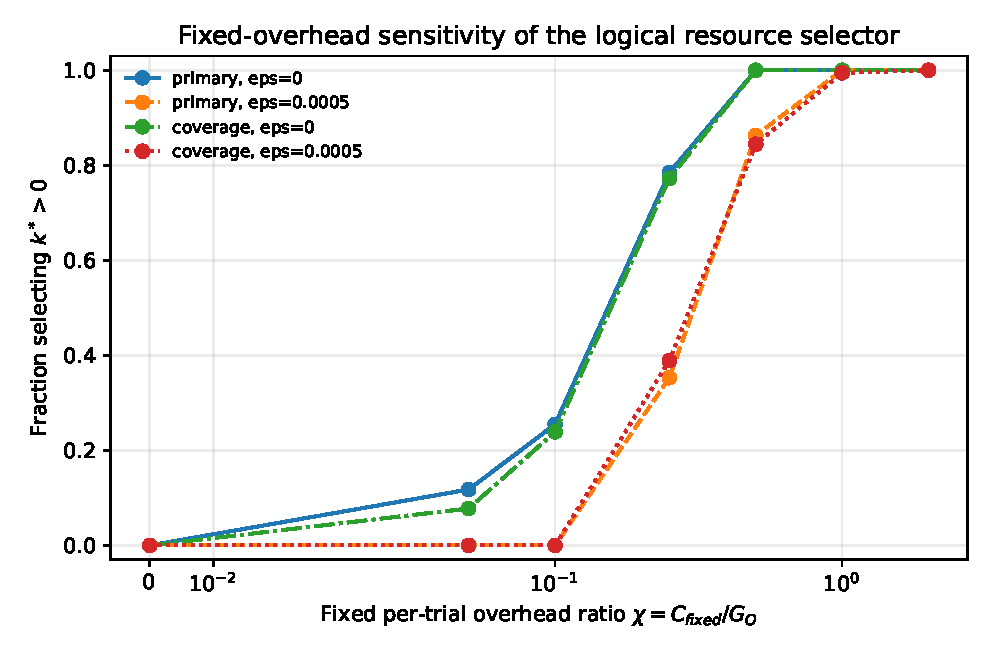
\includegraphics[width=0.86\linewidth]{../figures/fig_fixed_overhead_phase.pdf}
\caption{Fraction of feasible conditions selecting nonzero amplitude amplification as fixed per-trial overhead increases. The boundary is shown for the primary and coverage tiers at zero and maximum tested synthetic attenuation.}
\label{fig:fixedoverhead}
\end{figure}

\subsection{Amplitude-amplification sensitivity}
Figure~\ref{fig:aa} and Table~\ref{tab:aa} summarize the declared $q=0.95$ threshold reference over the 18 exact instances. At unit normalized oracle cost, the median selected $k^*$ is 5.0 at $\varepsilon_{\mathrm{model}}=0$, remains 5.0 at $5\times10^{-4}$ and $10^{-3}$, and decreases to 4.5 at $2\times10^{-3}$. With normalized oracle cost 8, the corresponding medians are 5.0, 5.0, 4.5, and 4.0. These depths are materially shallower than exact-optimum marking because the threshold oracle marks a larger, explicitly quality-conditioned set.

The oracle-cost effect remains instance dependent. The important change is semantic rather than merely numerical: $k^*$ is now selected for a declared quality threshold, so a reviewer can reproduce the marked-set rule from the cut-value comparator without assuming that the identities of optimum states are known in advance. The normalized oracle-cost sweep still does not substitute for compiling that comparator into reversible arithmetic.

\begin{figure}[t]
\centering
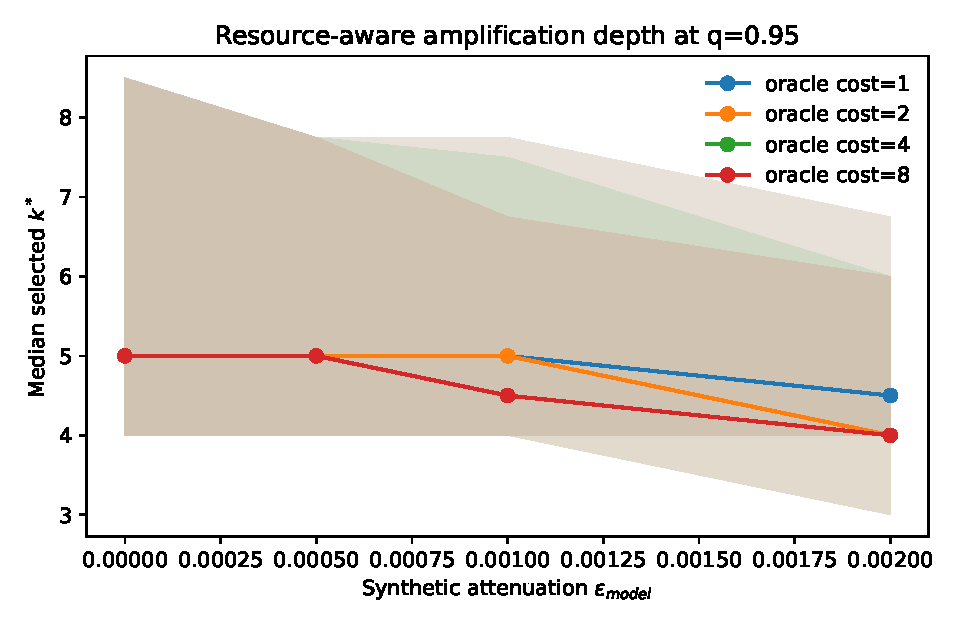
\includegraphics[width=0.82\linewidth]{../figures/fig_aa_sensitivity.pdf}
\caption{Median selected amplitude-amplification depth across 18 exact Max-Cut instances. Shaded regions show the interquartile range. Both attenuation and oracle cost are normalized sensitivity variables, not device measurements.}
\label{fig:aa}
\end{figure}

\begin{table}[t]
\centering
\caption{Aggregate amplitude-amplification sensitivity at the declared $q=0.95$ quality threshold. The complete machine-readable output also contains $q=0.90$ and $q=1.00$.}
\label{tab:aa}
\resizebox{\columnwidth}{!}{%
\begin{tabular}{rrrrr}
\toprule
$\varepsilon_{model}$ & oracle cost & median $k^*$ & IQR $k^*$ & median $\eta_{res}$ \\
\midrule
0.0000 & 1 & 5.0 & 4.0--8.5 & 0.141 \\
0.0000 & 2 & 5.0 & 4.0--8.5 & 0.206 \\
0.0000 & 4 & 5.0 & 4.0--8.5 & 0.334 \\
0.0000 & 8 & 5.0 & 4.0--8.5 & 0.591 \\
0.0005 & 1 & 5.0 & 4.0--7.8 & 0.152 \\
0.0005 & 2 & 5.0 & 4.0--7.8 & 0.222 \\
0.0005 & 4 & 5.0 & 4.0--7.8 & 0.360 \\
0.0005 & 8 & 5.0 & 4.0--7.8 & 0.637 \\
0.0010 & 1 & 5.0 & 4.0--7.8 & 0.164 \\
0.0010 & 2 & 5.0 & 4.0--7.8 & 0.239 \\
0.0010 & 4 & 4.5 & 4.0--7.5 & 0.387 \\
0.0010 & 8 & 4.5 & 4.0--6.8 & 0.684 \\
0.0020 & 1 & 4.5 & 4.0--6.8 & 0.189 \\
0.0020 & 2 & 4.0 & 4.0--6.8 & 0.273 \\
0.0020 & 4 & 4.0 & 3.0--6.0 & 0.440 \\
0.0020 & 8 & 4.0 & 3.0--6.0 & 0.776 \\
\bottomrule
\end{tabular}%
}

\end{table}

\subsection{Dense resource-uncertainty regions}
The threshold-aware dense uncertainty sweep contains 11,934 exact-instance conditions. At $q=0.90$, the median selected depth decreases from 3.0 to 2.0 across the attenuation endpoints, with the lower quartile reaching zero at $\varepsilon_{model}=0.003$; the median $\eta_{res}$ changes from 0.407 to 0.529. At $q=0.95$, the median selected depth decreases from 5.0 to 4.0 and the median $\eta_{res}$ changes from 0.265 to 0.395. At $q=1.00$, the median depth decreases from 9.0 to 6.0 while median $\eta_{res}$ changes from 0.149 to 0.312. Across all targets and resource coordinates, 13.3\% of conditions select $k^*=0$. Thus target strictness is itself a first-order configuration variable rather than a fixed background assumption.

\begin{figure}[t]
\centering
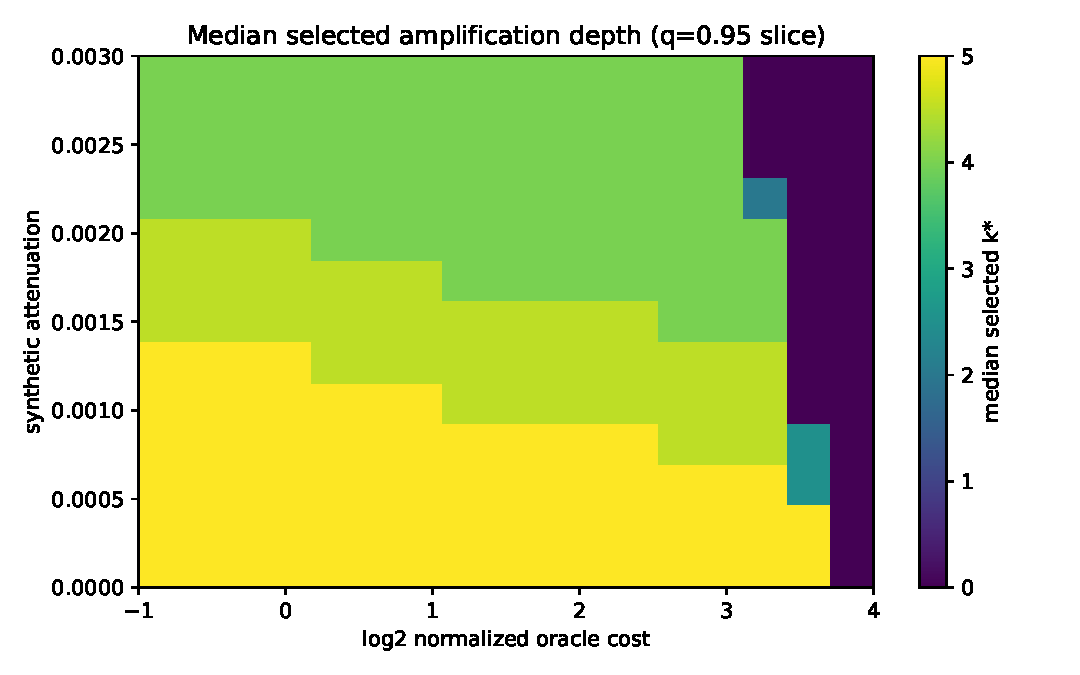
\includegraphics[width=0.82\linewidth]{../figures/fig_p2_robustness_map.pdf}
\caption{Dense resource-uncertainty map for the $q=0.95$ slice. Each cell is the median selected $k^*$ across the 18 exact instances; the machine-readable grid also contains $q=0.90$ and $q=1.00$. Both axes are model variables; neither is a device calibration.}
\label{fig:robustmap}
\end{figure}

\begin{table}[t]
\centering
\caption{Threshold-aware robustness summary at the attenuation endpoints, aggregated over the 18 exact instances and the normalized oracle-cost grid.}
\label{tab:robust}
\resizebox{\columnwidth}{!}{%
\begin{tabular}{rrrrr}
\toprule
target & $\varepsilon_{model}$ & median $k^*$ & IQR $k^*$ & median $\eta_{res}$ \\
\midrule
0.90 & 0.000 & 3.0 & 2.0--6.0 & 0.407 \\
0.90 & 0.003 & 2.0 & 0.0--3.0 & 0.529 \\
0.95 & 0.000 & 5.0 & 4.0--9.0 & 0.265 \\
0.95 & 0.003 & 4.0 & 2.0--5.0 & 0.395 \\
1.00 & 0.000 & 9.0 & 6.0--26.0 & 0.149 \\
1.00 & 0.003 & 6.0 & 3.2--9.0 & 0.312 \\
\bottomrule
\end{tabular}%
}

\end{table}

\subsection{Host simulation boundary and analytical large-space tier}
The reference implementation exhibits the expected rapid growth in classical simulation cost. At the two endpoint sizes, exact construction takes approximately 1 ms at $n=8$ and 0.70 s at $n=20$ on the recorded host, while a single fixed-parameter $p=1$ statevector evaluation rises from approximately 1 ms to 0.49 s. The two principal NumPy vectors used in this diagnostic grow from 0.004 MiB to 16 MiB. These timings define the evidence boundary of this implementation only; they do not measure quantum performance.

\begin{figure}[t]
\centering
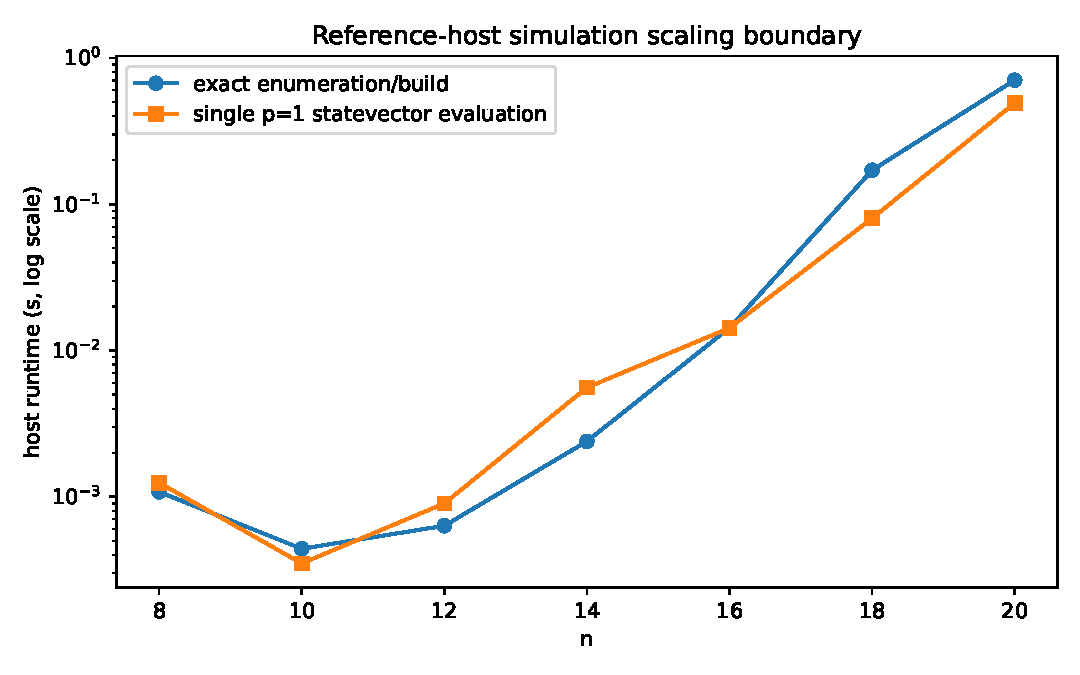
\includegraphics[width=0.82\linewidth]{../figures/fig_p2_simulator_scaling.pdf}
\caption{Host-side reference scaling for exact enumeration/build and one fixed-parameter $p=1$ statevector evaluation. The vertical axis is logarithmic.}
\label{fig:simscale}
\end{figure}

\begin{table}[t]
\centering
\caption{Host-side simulation-scaling diagnostic. Runtime and memory values characterize only the recorded reference implementation.}
\label{tab:simscale}
\resizebox{\columnwidth}{!}{%
\begin{tabular}{rrrrr}
\toprule
$n$ & states & exact-build (s) & $p=1$ eval. (s) & core memory (MiB) \\
\midrule
8 & 256 & 0.0011 & 0.0012 & 0.00 \\
10 & 1,024 & 0.0004 & 0.0003 & 0.02 \\
12 & 4,096 & 0.0006 & 0.0009 & 0.06 \\
14 & 16,384 & 0.0024 & 0.0056 & 0.25 \\
16 & 65,536 & 0.0143 & 0.0142 & 1.00 \\
18 & 262,144 & 0.1707 & 0.0801 & 4.00 \\
20 & 1,048,576 & 0.7046 & 0.4911 & 16.00 \\
\bottomrule
\end{tabular}%
}

\end{table}

The analytical Tier-III study demonstrates why resource assumptions become increasingly consequential when threshold-satisfying target events are rare. With one target-event state and zero attenuation, the median selected depth over the oracle-cost grid grows from 37 rounds for a $2^{12}$ search space to about 2,386 rounds for $2^{24}$. At $\varepsilon_{model}=0.003$, however, the median collapses to about 10 rounds across the larger modeled spaces. This is not a scalability claim for Max-Cut or a device forecast; it is a controlled sensitivity result showing that an attenuation penalty can dominate the ideal Grover-period scaling in the declared objective.

\begin{figure}[t]
\centering
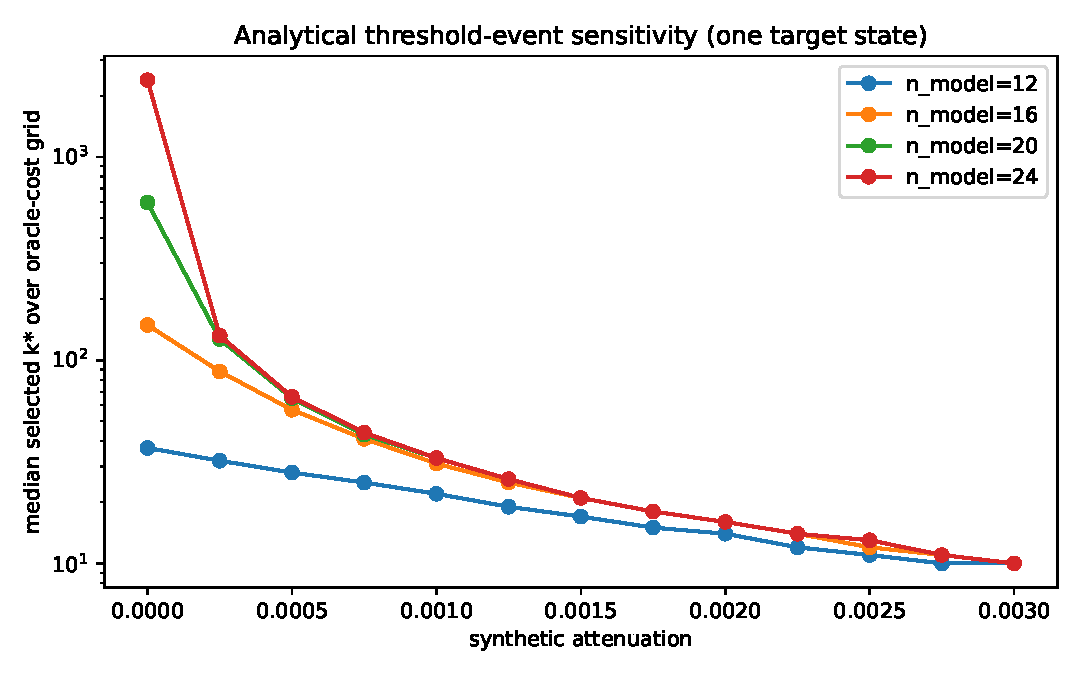
\includegraphics[width=0.82\linewidth]{../figures/fig_p2_large_tier.pdf}
\caption{Analytical large-search-space tier for one threshold-satisfying target-event state. Curves show the median selected $k^*$ over the normalized oracle-cost grid. These are abstract target-event calculations, not Max-Cut ground truth.}
\label{fig:largetier}
\end{figure}

\begin{table}[t]
\centering
\caption{Analytical threshold-event sensitivity at the attenuation endpoints.}
\label{tab:largetier}
\resizebox{\columnwidth}{!}{%
\begin{tabular}{rrrrr}
\toprule
$n_{model}$ & target-event states & $\varepsilon_{model}$ & median $k^*$ & IQR $k^*$ \\
\midrule
12 & 1 & 0.000 & 37.0 & 37.0--37.0 \\
12 & 1 & 0.003 & 10.0 & 9.0--10.0 \\
12 & 4 & 0.000 & 18.0 & 18.0--18.0 \\
12 & 4 & 0.003 & 8.0 & 8.0--8.0 \\
12 & 16 & 0.000 & 9.0 & 9.0--9.0 \\
12 & 16 & 0.003 & 6.0 & 6.0--6.0 \\
16 & 1 & 0.000 & 149.0 & 149.0--149.0 \\
16 & 1 & 0.003 & 10.0 & 10.0--11.0 \\
16 & 4 & 0.000 & 74.0 & 74.0--74.0 \\
16 & 4 & 0.003 & 10.0 & 10.0--10.0 \\
16 & 16 & 0.000 & 37.0 & 37.0--37.0 \\
16 & 16 & 0.003 & 10.0 & 9.0--10.0 \\
20 & 1 & 0.000 & 596.0 & 596.0--596.0 \\
20 & 1 & 0.003 & 10.0 & 10.0--11.0 \\
20 & 4 & 0.000 & 298.0 & 298.0--298.0 \\
20 & 4 & 0.003 & 10.0 & 10.0--11.0 \\
20 & 16 & 0.000 & 149.0 & 149.0--149.0 \\
20 & 16 & 0.003 & 10.0 & 10.0--11.0 \\
24 & 1 & 0.000 & 2386.0 & 2386.0--2387.0 \\
24 & 1 & 0.003 & 10.0 & 10.0--11.0 \\
24 & 4 & 0.000 & 1193.0 & 1193.0--1193.0 \\
24 & 4 & 0.003 & 10.0 & 10.0--11.0 \\
24 & 16 & 0.000 & 596.0 & 596.0--596.0 \\
24 & 16 & 0.003 & 10.0 & 10.0--11.0 \\
\bottomrule
\end{tabular}%
}

\end{table}

\subsection{Benchmark-normalized calibration targets across methods}
As a complementary exact-tier calibration, the benchmark reports the same event
\begin{equation}
P_{\tau_q}=\Pr[C(x)\geq\tau_q]
\end{equation}
for uniform sampling, the reference amplitude-amplification operating point ($\varepsilon_{model}=0$, unit normalized oracle cost), multistart hill climbing, fixed-budget simulated annealing, fixed-budget tabu search, and each tested QAOA depth. This is a common success target, not a claim that a QAOA evaluation, a classical objective evaluation, and an amplitude-amplification resource unit have equal physical cost.

Across all 18 primary instances, the median target-hit probabilities at $q=0.95$ are 0.0105 for uniform sampling, 0.8399 for the query-level amplitude-amplification reference, 0.6875 for hill climbing, 1.000 for simulated annealing, 1.000 for tabu search, and 0.0115, 0.0123, and 0.0124 for QAOA depths $p=1,2,3$. The two fixed-budget classical heuristics also have median target-hit fraction 1.000 at $q=0.90$ and $q=1.00$. Thus the stronger classical references dominate the common target-hit statistic on these micro-instances. The probabilities still do not establish comparative runtime advantage because the method-specific resource units are intentionally not merged.

\begin{figure}[t]
\centering
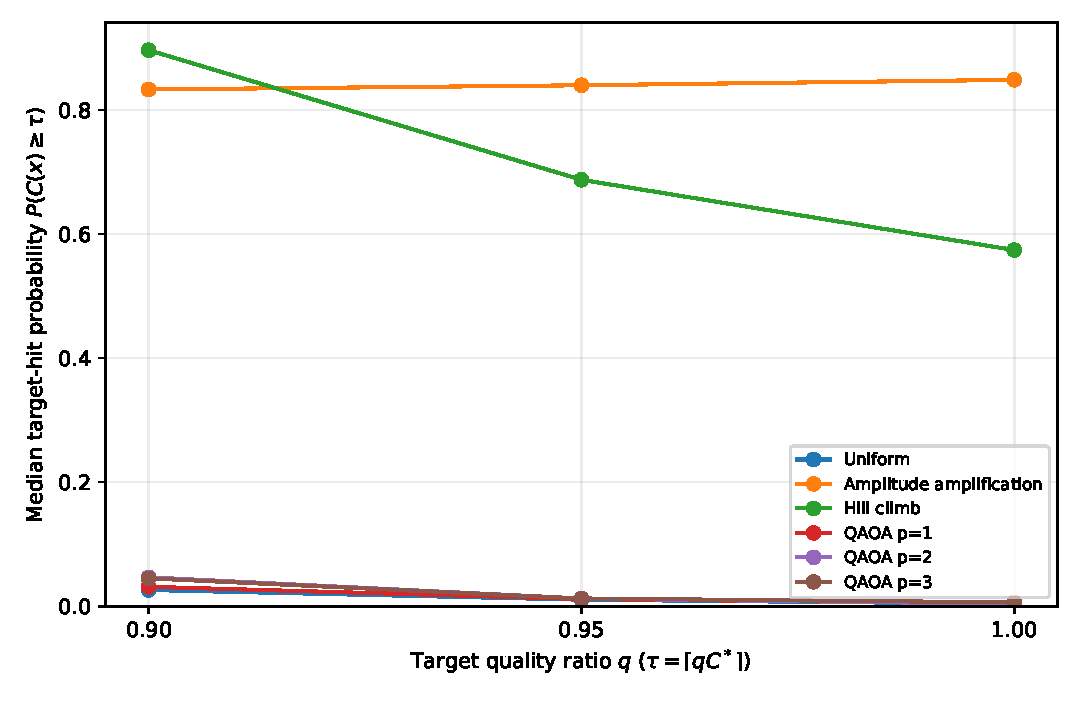
\includegraphics[width=0.82\linewidth]{../figures/fig_threshold_common_metric.pdf}
\caption{Core target-hit probability view on the 18 primary instances. The target event is identical, $C(x)\geq\tau_q$, while method-specific execution costs remain deliberately unmerged. The fixed-budget simulated-annealing and tabu-search references are reported separately in the classical-reference table and machine-readable ledger.}
\label{fig:targetmetric}
\end{figure}

\begin{table}[t]
\centering
\caption{Median target-hit probability for the core quantum/uniform/hill-climb view on the 18 primary instances. AA denotes the query-level reference operating point with zero synthetic attenuation and unit normalized oracle cost; stronger fixed-budget classical references are reported separately.}
\label{tab:targetmetric}
\resizebox{\columnwidth}{!}{%
\begin{tabular}{rrrrrrr}
\toprule
target & uniform & AA & hill climb & QAOA $p=1$ & $p=2$ & $p=3$ \\
\midrule
0.90 & 0.0261 & 0.8331 & 0.8965 & 0.0378 & 0.0387 & 0.0480 \\
0.95 & 0.0105 & 0.8399 & 0.6875 & 0.0097 & 0.0136 & 0.0151 \\
1.00 & 0.0039 & 0.8487 & 0.5742 & 0.0033 & 0.0041 & 0.0074 \\
\bottomrule
\end{tabular}%
}

\end{table}

\subsection{QAOA depth and optimizer variability}
Of the 270 QAOA optimization runs, 269 return a successful optimizer convergence flag. The aggregate results are shown in Table~\ref{tab:qaoa} and Figure~\ref{fig:qaoa}. The median of the 18 instance-level median approximation ratios is 0.655 at $p=1$, 0.697 at $p=2$, and 0.700 at $p=3$. The aggregate central statistic increases from $p=1$ to the two deeper settings, but the difference between $p=2$ and $p=3$ is small.

The median of instance-level median optimum-state probabilities is 0.00441, 0.00380, and 0.00611 for $p=1,2,3$. These probabilities have wide between-instance and between-seed variation. Ten of the 18 instances attain their best median approximation ratio at $p=3$, whereas eight favor $p=2$. This is a more cautious result than identifying one universal QAOA depth.

The best single run in the complete statevector sweep occurs for instance \texttt{n8\_d25\_s42} at $p=3$ and optimizer seed 1, with approximation ratio 0.9524 and exact optimum-state probability 0.2287. This best-run value is retained in the raw ledger but is not used as the representative result.

\begin{figure}[t]
\centering
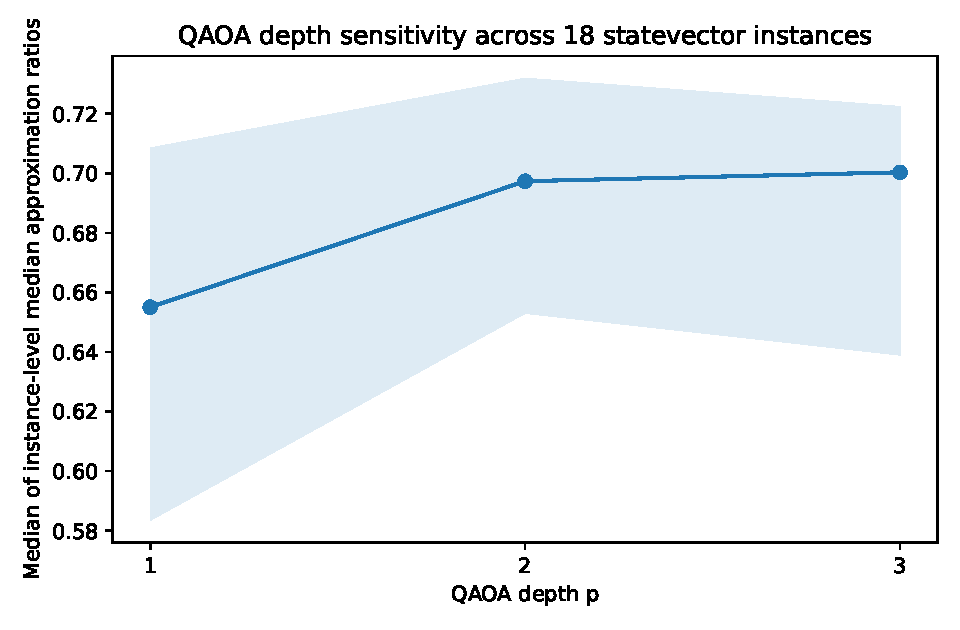
\includegraphics[width=0.82\linewidth]{../figures/fig_qaoa_depth.pdf}
\caption{QAOA depth sensitivity across 18 exact instances. The line shows the median of instance-level median approximation ratios; the band shows the interquartile range across instances. Each instance-level median is computed from five independent optimizer initializations.}
\label{fig:qaoa}
\end{figure}

\begin{table}[t]
\centering
\caption{Aggregate ideal-statevector QAOA results. Each depth contains 18 instances and five optimizer starts per instance.}
\label{tab:qaoa}
\resizebox{\columnwidth}{!}{%
\begin{tabular}{rrrrr}
\toprule
$p$ & instances & runs & median instance AR & median instance $P_{opt}$ \\
\midrule
1 & 18 & 90 & 0.673 & 0.0033 \\
2 & 18 & 90 & 0.689 & 0.0041 \\
3 & 18 & 90 & 0.716 & 0.0074 \\
\bottomrule
\end{tabular}%
}

\end{table}

The equal-cap optimizer ablation gives a different but complementary view. Under the 128-objective-evaluation cap, the median of the 18 instance-level median approximation ratios for L-BFGS-B is 0.655, 0.698, and 0.697 at $p=1,2,3$, respectively; the corresponding COBYLA values are 0.691, 0.700, and 0.722. On the 90 paired $(\text{instance},\text{seed})$ comparisons per depth, COBYLA attains the larger approximation ratio in 62/90, 47/90, and 59/90 pairs for $p=1,2,3$. These are descriptive paired counts rather than significance claims.

The cap is materially active. The fraction of runs ending at the evaluation ceiling for L-BFGS-B is 0.000, 0.378, and 0.744 across $p=1,2,3$; for COBYLA it is 0.489, 0.989, and 0.989. Thus the ablation should be interpreted as attained quality under a finite optimization budget, not as a comparison of fully converged optimizers. In particular, the higher COBYLA medians in this budgeted experiment do not establish optimizer superiority outside this suite or budget.

\begin{table}[t]
\centering
\caption{Paired ideal-statevector QAOA optimizer robustness under a common cap of 128 exact expectation-objective evaluations per run. ``Budget-exhaust.'' is the fraction of runs that end at the cap without an earlier successful optimizer termination.}
\label{tab:qaoaoptbudget}
\resizebox{\columnwidth}{!}{%
\begin{tabular}{lrrrrr}
\toprule
optimizer & $p$ & runs & median inst. AR & median evals & budget-exhaust. \\
\midrule
L-BFGS-B & 1 & 90 & 0.655 & 39 & 0.000 \\
L-BFGS-B & 2 & 90 & 0.698 & 115 & 0.378 \\
L-BFGS-B & 3 & 90 & 0.697 & 128 & 0.744 \\
COBYLA & 1 & 90 & 0.691 & 125 & 0.489 \\
COBYLA & 2 & 90 & 0.700 & 128 & 0.989 \\
COBYLA & 3 & 90 & 0.722 & 128 & 0.989 \\
\bottomrule
\end{tabular}%
}

\end{table}


\subsection{Instance-clustered inferential checks}
The fixed-suite inferential analysis supports a narrower statement than the descriptive aggregate medians alone. For the primary L-BFGS-B depth study, the Friedman statistic across the 18 matched instance medians is $\chi_F^2=13.768$ with $p=0.00102$. After Holm correction, both $p=2$ versus $p=1$ and $p=3$ versus $p=1$ remain below 0.05. Their median paired approximation-ratio differences are $+0.0162$ and $+0.0084$, with instance-bootstrap 95\% intervals $[0.0065,0.0612]$ and $[0.0014,0.0333]$, respectively; both have $p_{\rm Holm}=0.0101$. The $p=3$ versus $p=2$ contrast has median $+0.0067$, interval $[-0.0085,0.0252]$, and $p_{\rm Holm}=0.7337$. Thus the fixed suite supports a depth effect relative to $p=1$ but does not distinguish the two deeper settings after multiplicity correction.

For the 128-evaluation optimizer ablation, the primary paired unit is also the instance: the five seed-level COBYLA-minus-L-BFGS-B differences are first reduced to an instance median. The median instance differences are $+0.0122$, $-0.0001$, and $+0.0335$ at $p=1,2,3$. Their Holm-adjusted signed-rank $p$ values are 0.0003, 0.7660, and 0.0013, respectively. The 95\% bootstrap intervals exclude zero at $p=1$ and $p=3$ but include zero at $p=2$. Consequently, this fixed 128-evaluation budget supports attained-quality differences favoring COBYLA at $p=1$ and $p=3$ within the fixed suite, not a general optimizer-convergence ranking. Table~\ref{tab:qaoainference} reports the paired effect sizes and intervals.

\begin{table}[t]
\centering
\caption{Instance-clustered inferential checks for QAOA depth and optimizer family. Five optimizer starts are collapsed within each of the 18 fixed primary benchmark instances before testing. Confidence intervals resample instances; $p$ values are Holm-adjusted within the three depth contrasts or the three optimizer contrasts.}
\label{tab:qaoainference}
\resizebox{\columnwidth}{!}{%
\begin{tabular}{lrrrrr}
\toprule
\multicolumn{6}{l}{\textit{Depth contrasts}} \\
contrast & median $\Delta$ & 95\% CI & $p_{\rm Holm}$ & $r_{\rm rb}$ & $n$ \\
\midrule
p2-p1 & +0.0234 & [+0.0045,+0.0648] & 0.0080 & +0.731 & 18 \\
p3-p1 & +0.0379 & [+0.0179,+0.1369] & 0.0002 & +0.942 & 18 \\
p3-p2 & +0.0307 & [+0.0045,+0.0428] & 0.0080 & +0.743 & 18 \\
\midrule
\multicolumn{6}{l}{\textit{Optimizer contrasts: COBYLA $-$ L-BFGS-B}} \\
$p$ & median $\Delta$ & 95\% CI & $p_{\rm Holm}$ & $r_{\rm rb}$ & $n$ \\
\midrule
1 & +0.0015 & [-0.0000,+0.0281] & 0.0911 & +0.556 & 18 \\
2 & +0.0018 & [-0.0001,+0.0086] & 0.0911 & +0.462 & 18 \\
3 & +0.0084 & [-0.0007,+0.0175] & 0.0911 & +0.579 & 18 \\
\bottomrule
\end{tabular}%
}

\end{table}

\subsection{Classical references and interpretation boundary}
The simple hill-climbing sanity reference is already strong on these micro-instances. Across all six instances for each size, its median local-search approximation ratio is 1.000 for $n=8$, 1.000 for $n=10$, and 0.977 for $n=12$, with median optimum-hit fractions 0.613, 0.613, and 0.387. The stronger fixed-budget references sharpen that conclusion. For both simulated annealing and tabu search, the median of the instance-level median run-best approximation ratios is 1.000 at $n=8,10,12$, and the median optimum-hit fraction across the six instances at each size is also 1.000. Simulated annealing solves every instance in every recorded run (minimum instance-level optimum-hit fraction 1.000), whereas tabu search has a worst instance-level fraction of 0.359; nevertheless, every one of the 18 instances is solved exactly by at least one of the 64 runs of each method.

Figure~\ref{fig:classical} retains the original sanity comparison between the best QAOA depth by instance-level median and hill climbing. The fixed-budget results in Table~\ref{tab:classicalbudget} provide the stronger classical context. Consequently, the present data do not support a performance-advantage claim for QAOA or for the amplitude-amplification formulation. Instead, they show that these exact micro-instances are classically easy under multiple reproducible heuristics, so the quantum-side experiments should be interpreted as configuration diagnostics rather than competitiveness evidence.

\begin{figure}[t]
\centering
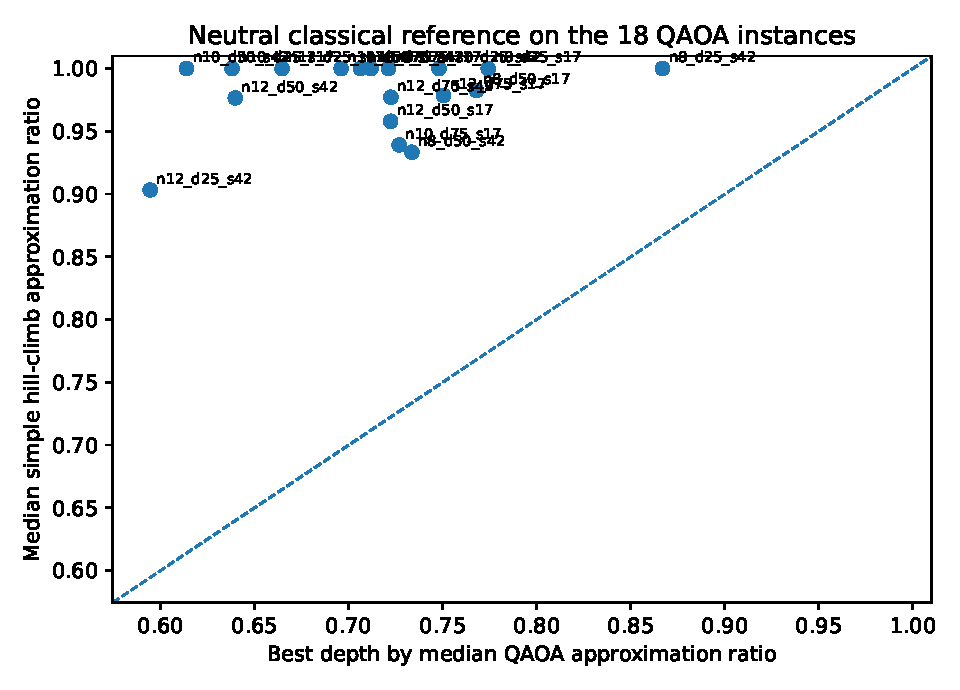
\includegraphics[width=0.82\linewidth]{../figures/fig_qaoa_vs_local.pdf}
\caption{Neutral classical reference on the 18 QAOA instances. The horizontal coordinate is the best QAOA depth chosen by median approximation ratio for each instance; the vertical coordinate is the median approximation ratio of the simple multistart hill climber. The dashed line denotes equality.}
\label{fig:classical}
\end{figure}

\begin{table}[t]
\centering
\caption{Simple classical hill-climbing reference aggregated by graph size. These values are included as a sanity baseline, not as a best-known classical bound.}
\label{tab:classical}
\resizebox{\columnwidth}{!}{%
\begin{tabular}{rrrr}
\toprule
$n$ & instances & median local-search ratio & median optimum-hit fraction \\
\midrule
8 & 6 & 1.000 & 0.613 \\
10 & 6 & 1.000 & 0.613 \\
12 & 6 & 0.977 & 0.387 \\
\bottomrule
\end{tabular}%
}

\end{table}

\begin{table}[t]
\centering
\caption{Fixed-objective-evaluation-budget classical references. Each method uses 64 independent runs per instance and at most 4096 complete objective evaluations per run. Exact $C^*$ is used only for retrospective scoring.}
\label{tab:classicalbudget}
\resizebox{\columnwidth}{!}{%
\begin{tabular}{lrrrrr}
\toprule
method & $n$ & inst. & eval. cap & median AR & opt.-hit frac. \\
\midrule
sim. annealing & 8 & 6 & 4096 & 1.000 & 1.000 \\
sim. annealing & 10 & 6 & 4096 & 1.000 & 1.000 \\
sim. annealing & 12 & 6 & 4096 & 1.000 & 1.000 \\
tabu search & 8 & 6 & 4096 & 1.000 & 1.000 \\
tabu search & 10 & 6 & 4096 & 1.000 & 1.000 \\
tabu search & 12 & 6 & 4096 & 1.000 & 0.961 \\
\bottomrule
\end{tabular}%
}

\end{table}

\section{Discussion}
\subsection{What the resource model shows}
The amplitude-amplification results show that a stopping rule based only on ideal rotation geometry is incomplete for a resource-aware workflow. More importantly, the operational construction separates the question ``what target should be marked?'' from knowledge of $C^*$. The oracle is defined by a cut-value comparator, while Eq.~\eqref{eq:operthreshold} fixes its threshold from graph-observable anchors. Exact enumeration is then used only to audit feasibility and marked fraction. The $C^*$-normalized $q$ axis remains useful as a calibration experiment, but it is no longer conflated with deployable threshold construction.

The normalized-cost grid therefore remains a sensitivity statement rather than a processor model. The architecture-informed oracle layer sharpens this interpretation: once a concrete ripple-style accumulator/comparator burden is charged and its logical depth is coupled to attenuation, the selector chooses no amplification in all 255 operational conditions when fixed per-trial work is set to zero. The P0-2 stress test shows why this boundary must be stated: the median zero-attenuation break-even fixed overhead is only 0.163 oracle-cost units in the primary tier, and nonzero amplification becomes common by $\chi=0.25$. The result is therefore a conditional configuration map, not a claim that amplitude amplification is generally useless. A compiler-locked study may replace the logical template and synthetic overhead with target-specific gate counts, fixed control/readout/verification costs, depth, and duration without changing that evidence boundary.

\subsection{What the QAOA results show}
The QAOA experiment reinforces the distinction between depth capacity and attained performance. The aggregate median approximation ratio rises from $p=1$ to $p=2$ and changes only slightly from $p=2$ to $p=3$ in this limited suite; corrected paired inference supports both deeper settings over $p=1$ but does not distinguish $p=3$ from $p=2$. More importantly, the spread across random initializations means that a single run is not a stable basis for comparison. The paired 128-evaluation ablation adds a second sensitivity axis: COBYLA has higher aggregate medians than L-BFGS-B at all three tested depths, but many $p=2$ and $p=3$ runs reach the cap, so the result is explicitly a finite-budget optimizer comparison rather than a convergence ranking. This is consistent with prior work on optimizer and initialization sensitivity \cite{fernandez2022,sack2021}.

The benchmark therefore treats optimizer seed as an experimental factor, not an implementation detail. A hardware extension should retain the same discipline and additionally separate optimization shots, final evaluation shots, compiler seed, device calibration state, and queue/execution timing.

\subsection{Why the classical reference matters}
The classical references prevent a misleading interpretation of micro-instance quantum results. The simple hill climber is frequently exact, and both fixed-budget simulated annealing and tabu search have median run-best approximation ratio 1.000 with median optimum-hit fraction 1.000 at every tested size. This finding is not a failure of the benchmark; it is precisely why neutral baselines are necessary. A quantum method should not be described as advantageous simply because it improves over uniform sampling or because its internal hit probability increases when multiple transparent classical heuristics already solve the same small instances reliably.

The current study therefore separates two questions that are often conflated. The first is a configuration question: how do quantum algorithm parameters respond to target quality and resource assumptions? The second is a comparative-performance question: does the resulting workflow outperform suitable classical alternatives under matched physical resources? The common $P_{\tau}$ metric aligns the success event but does not solve the second problem because physical costs remain unmatched. The present results therefore strengthen fairness of interpretation without converting the study into a performance-advantage claim.

\subsection{Relevance to future-generation quantum systems}
The systems relevance lies in the explicit interface between algorithmic parameters and resource assumptions. Hybrid quantum platforms must eventually map abstract oracle calls, variational layers, classical control, and scheduling into concrete execution resources. Recent FGCS work emphasizes precisely this quantum--classical integration, simulation, and infrastructure perspective \cite{markidis2026editorial,netzer2026,vallero2026}. The current benchmark provides a small, fully auditable layer beneath such system studies: exact problem ground truth, reproducible parameter sweeps, a separate seed/topology coverage stress test, and a claim policy that prevents model variables from being relabeled as empirical hardware measurements. The additional coverage tier is deliberately kept separate from the 18-instance primary QAOA inference so that broader descriptive stress testing does not retroactively inflate the inferential sample.

\section{Threats to validity and limitations}
The exact-comparison tier is intentionally small in vertex count. Exact ground truth remains restricted to at most 12 vertices, so no Max-Cut scaling claim follows from the observed approximation ratios or optimum-state probabilities. The separate $n=14$--20 host-simulation diagnostic measures classical reference cost only, and the $n_{model}=12$--24 analytical tier uses abstract marked fractions rather than Max-Cut optima. These tiers expand the evidence boundary without pretending that extrapolative model rows are exact optimization results. Seed/topology coverage is broader than in the primary design---five random seeds and three structured families produce 63 exact coverage instances---but it is still a deliberately finite, hand-declared benchmark rather than a probability sample over graph populations. The structured families use only two weight seeds, and no claim is made that cycle, 3-regular circulant, and two-community graphs exhaust relevant Max-Cut topology classes.

The amplitude-amplification oracle now marks a numeric threshold event $C(x)\geq\tau$ rather than a pre-enumerated optimum set. The operational threshold in Eq.~\eqref{eq:operthreshold} does not use $C^*$. The marked-fraction experiment in Eq.~\eqref{eq:rhoretention} quantifies the consequence of multiplicative error in $\rho_\tau$, but it does not supply a physical estimator or an estimator-free unknown-solution-count schedule. Exact $\rho_\tau$ therefore remains a retrospective reference, not a deployable information assumption. The study now includes a reversible weighted-cut accumulator/comparator resource template, but its Toffoli, CNOT, ancilla, and logical-depth counts remain architecture-informed bookkeeping rather than compiler output. The factor used to form $G_{\rm eq}$ is a transparent weighting convention, not a physical native-gate equivalence. Connectivity, routing, synthesis choice, fault-tolerant realization, and backend timing can change the concrete cost. The attenuation variables are synthetic; neither the abstract $D_{\mathrm{prep}},D_{\mathrm{iter}}$ sensitivity coordinates nor the architecture-coupled $\varepsilon_D$ are measured device quantities. The fixed-overhead coordinate $\chi=C_{\rm fixed}/G_{\mathcal O}$ is likewise synthetic: it demonstrates sensitivity to omitted per-trial work but does not estimate control, measurement, verification, network, queue, or host-device handoff cost on any platform.

The QAOA experiments use exact statevectors. The primary depth study uses L-BFGS-B, while the optimizer ablation compares L-BFGS-B with COBYLA under one finite cap of 128 exact expectation evaluations and five paired initializations. The statistical layer collapses repeated starts within each of the 18 primary instances and therefore avoids treating optimizer seeds as independent graph replicates; nevertheless, 18 fixed instances still provide limited inferential resolution and do not support population-level generalization. This broadens the optimizer evidence but still does not characterize the full optimization landscape, and the cap binds many $p=2$ and $p=3$ runs. Hardware noise, finite-shot optimization, parameter-transfer methods, alternative mixers, advanced initialization strategies, and additional optimizer families remain outside the current evidence set. The classical layer now contains hill climbing, simulated annealing, and tabu search, but it is still not a comprehensive classical benchmark: no semidefinite Goemans--Williamson implementation, branch-and-bound timing study, or large-instance heuristic competition is claimed \cite{goemans1995}. Exact enumeration supplies micro-instance ground truth and is not presented as a scalable competitor.

Finally, the benchmark does not compare physical energy consumption, monetary cost, or elapsed quantum-service time. Those quantities require a different evidence layer with explicit backend and system telemetry.

\section{Conclusion}
This paper presented a reproducible benchmark for threshold-oriented resource-aware amplitude amplification and QAOA with explicitly separated exact, host-simulation, and analytical tiers. The main threshold-construction result is operational rather than optimum-normalized: $\tau_\lambda^{\rm op}$ is built from the uniform-random expected cut and a Laplacian spectral upper bound without using $C^*$. Retrospective exact validation shows that $\lambda=0.25$ and $0.40$ are feasible on all 18 primary benchmark instances, whereas $\lambda=0.55$ is feasible on 15/18, making target infeasibility visible instead of silently assuming attainability. A separate exact coverage stress test broadens the seed set and adds cycle, 3-regular circulant, and two-community topologies: the first operational level is feasible on all 63 coverage instances, the second on 62/63, the strictest level on 55/63, and all 360 architecture-coupled feasible coverage conditions at $\varepsilon_D\in\{0,10^{-3}\}$ retain $k^*=0$ under the zero-fixed-overhead convention. A separate 8,085-condition fixed-overhead stress test shows that the zero-round conclusion is conditional: at zero attenuation, median break-even overhead ratios are 0.163 and 0.168 oracle-cost units for the primary and coverage tiers. A separate $C^*$-normalized calibration study contains 864 coarse and 11,934 dense sensitivity conditions and confirms that target strictness, synthetic attenuation, and normalized oracle cost materially change the selected amplification depth. Across 18 statevector QAOA instances and 270 primary L-BFGS-B optimization runs, aggregate median approximation ratios are 0.655/0.697/0.700 at $p=1/2/3$. A separate 540-run paired optimizer ablation under a 128-objective-evaluation cap yields aggregate medians of 0.655/0.698/0.697 for L-BFGS-B and 0.691/0.700/0.722 for COBYLA, while also showing substantial cap exhaustion at the deeper settings. Instance-clustered inference further narrows the interpretation: the depth omnibus test is significant on the fixed suite ($p=0.00102$); both $p=2$ versus $p=1$ and $p=3$ versus $p=1$ survive Holm correction ($p_{\rm Holm}=0.0101$), whereas $p=3$ versus $p=2$ does not. Under the finite optimizer budget, COBYLA-minus-L-BFGS-B contrasts survive correction at $p=1$ and $p=3$ but not at $p=2$; this remains a budget-conditioned attained-quality result rather than a general optimizer ranking. The classical conclusion remains strong: simulated annealing and tabu search both attain a median run-best ratio and median optimum-hit fraction of 1.000 at every tested size, reinforcing that these micro-instances are configuration tests rather than evidence for quantum competitiveness.

The primary contribution is therefore a benchmark discipline rather than a speedup claim: construct operational thresholds without $C^*$, distinguish threshold construction from exact-tier validation, quantify stopping-depth regret under marked-fraction misspecification, align methods on a common target-hit event, and then test whether conclusions survive an explicit reversible-oracle burden. In the architecture-informed logical layer developed here, the oracle median grows from 420 to 1,088 modeled Toffoli gates across $n=8$ to $12$, and all 255 coupled operational conditions select the no-amplification configuration when fixed per-trial overhead is zero. The fixed-overhead phase boundary is retained alongside this negative result because it shows exactly where that configuration conclusion changes rather than treating one bookkeeping convention as universal. Compiler-locked measurements can replace the logical template in a subsequent evidence layer without being retroactively labeled as present evidence.

\section*{Data and code availability}
All primary and expanded coverage benchmark instances, machine-readable edge ledgers, exact ground-truth records, operational and benchmark-normalized threshold definitions, retrospective operational-feasibility records, marked-fraction misspecification rows, common target-metric rows, raw QAOA runs, paired optimizer-budget runs and summaries, instance-clustered inferential ledgers, raw and summarized fixed-budget classical runs, analytical sensitivity outputs, generated tables, test results, the exact environment lock, the automated preflight validator, and a hash-bearing run manifest are included in the accompanying reproducibility package.

\section*{Funding}
This research did not receive any specific grant from funding agencies in the public, commercial, or not-for-profit sectors.

\section*{Declaration of competing interest}
The author declares no known competing financial interests or personal relationships that could have appeared to influence the work reported in this paper.

\section*{CRediT authorship contribution statement}
Ercan Erkalkan: Conceptualization, Methodology, Software, Validation, Formal analysis, Investigation, Data curation, Visualization, Writing -- original draft, Writing -- review and editing, Project administration.

\section*{Declaration of generative AI and AI-assisted technologies in the manuscript preparation process}
During the preparation of this work, the author used OpenAI ChatGPT for manuscript organization, drafting and language refinement, code drafting, test design, literature-navigation support, and consistency checking. The final audit and revision used ChatGPT with GPT-5.6 Sol on 31 August 2026; exact model-version identifiers for earlier ChatGPT-assisted sessions were not consistently recorded and are therefore not inferred retrospectively. After using this tool, the author reviewed and edited the content as needed, executed and verified the computational workflow and reported outputs, checked the cited sources, and takes full responsibility for the content of the publication.

\bibliographystyle{elsarticle-num}
\bibliography{references}

\end{document}
